
\section{Results}
\noindent
We generated the visibility graph characteristics for three tectonic seismic regions in northern Iran for the period from 2005 to 2015. Number of earthquake in each catalog after declustering and the seismicity parameters are presented in Table.~\ref{tab:b_k_m_param}. 


\begin{table}[h]
\centering
\caption{Seismic parameters and K-M slope values for north Iran tectonic seismic zones.}
\begin{tabular}{ccccc}
Region          & Number of Earthquake &  Mc &  b-value & K-M slope \\ \hline
Azerbaijan     & 93                                 & 3.5   & 1.0190  & 9.2004       \\ \hline
Alborz            & 488                               & 2.9   & 0.8532  & 9.2821      \\ \hline
Kopek Dagh  & 282                               & 2.6   & 0.5799  & 6.5818     \\ \hline
\end{tabular}
\label{tab:b_k_m_param}
\end{table}

\noindent
Fig.~\ref{fig:k_m_plot_m} shows the $k-M$ relationship for the study regions.  In general with increasing magnitude the connectivity degree increases which results in increasing the slope of the $k-M$ relationship. 

\begin{figure} [ht]
\centering
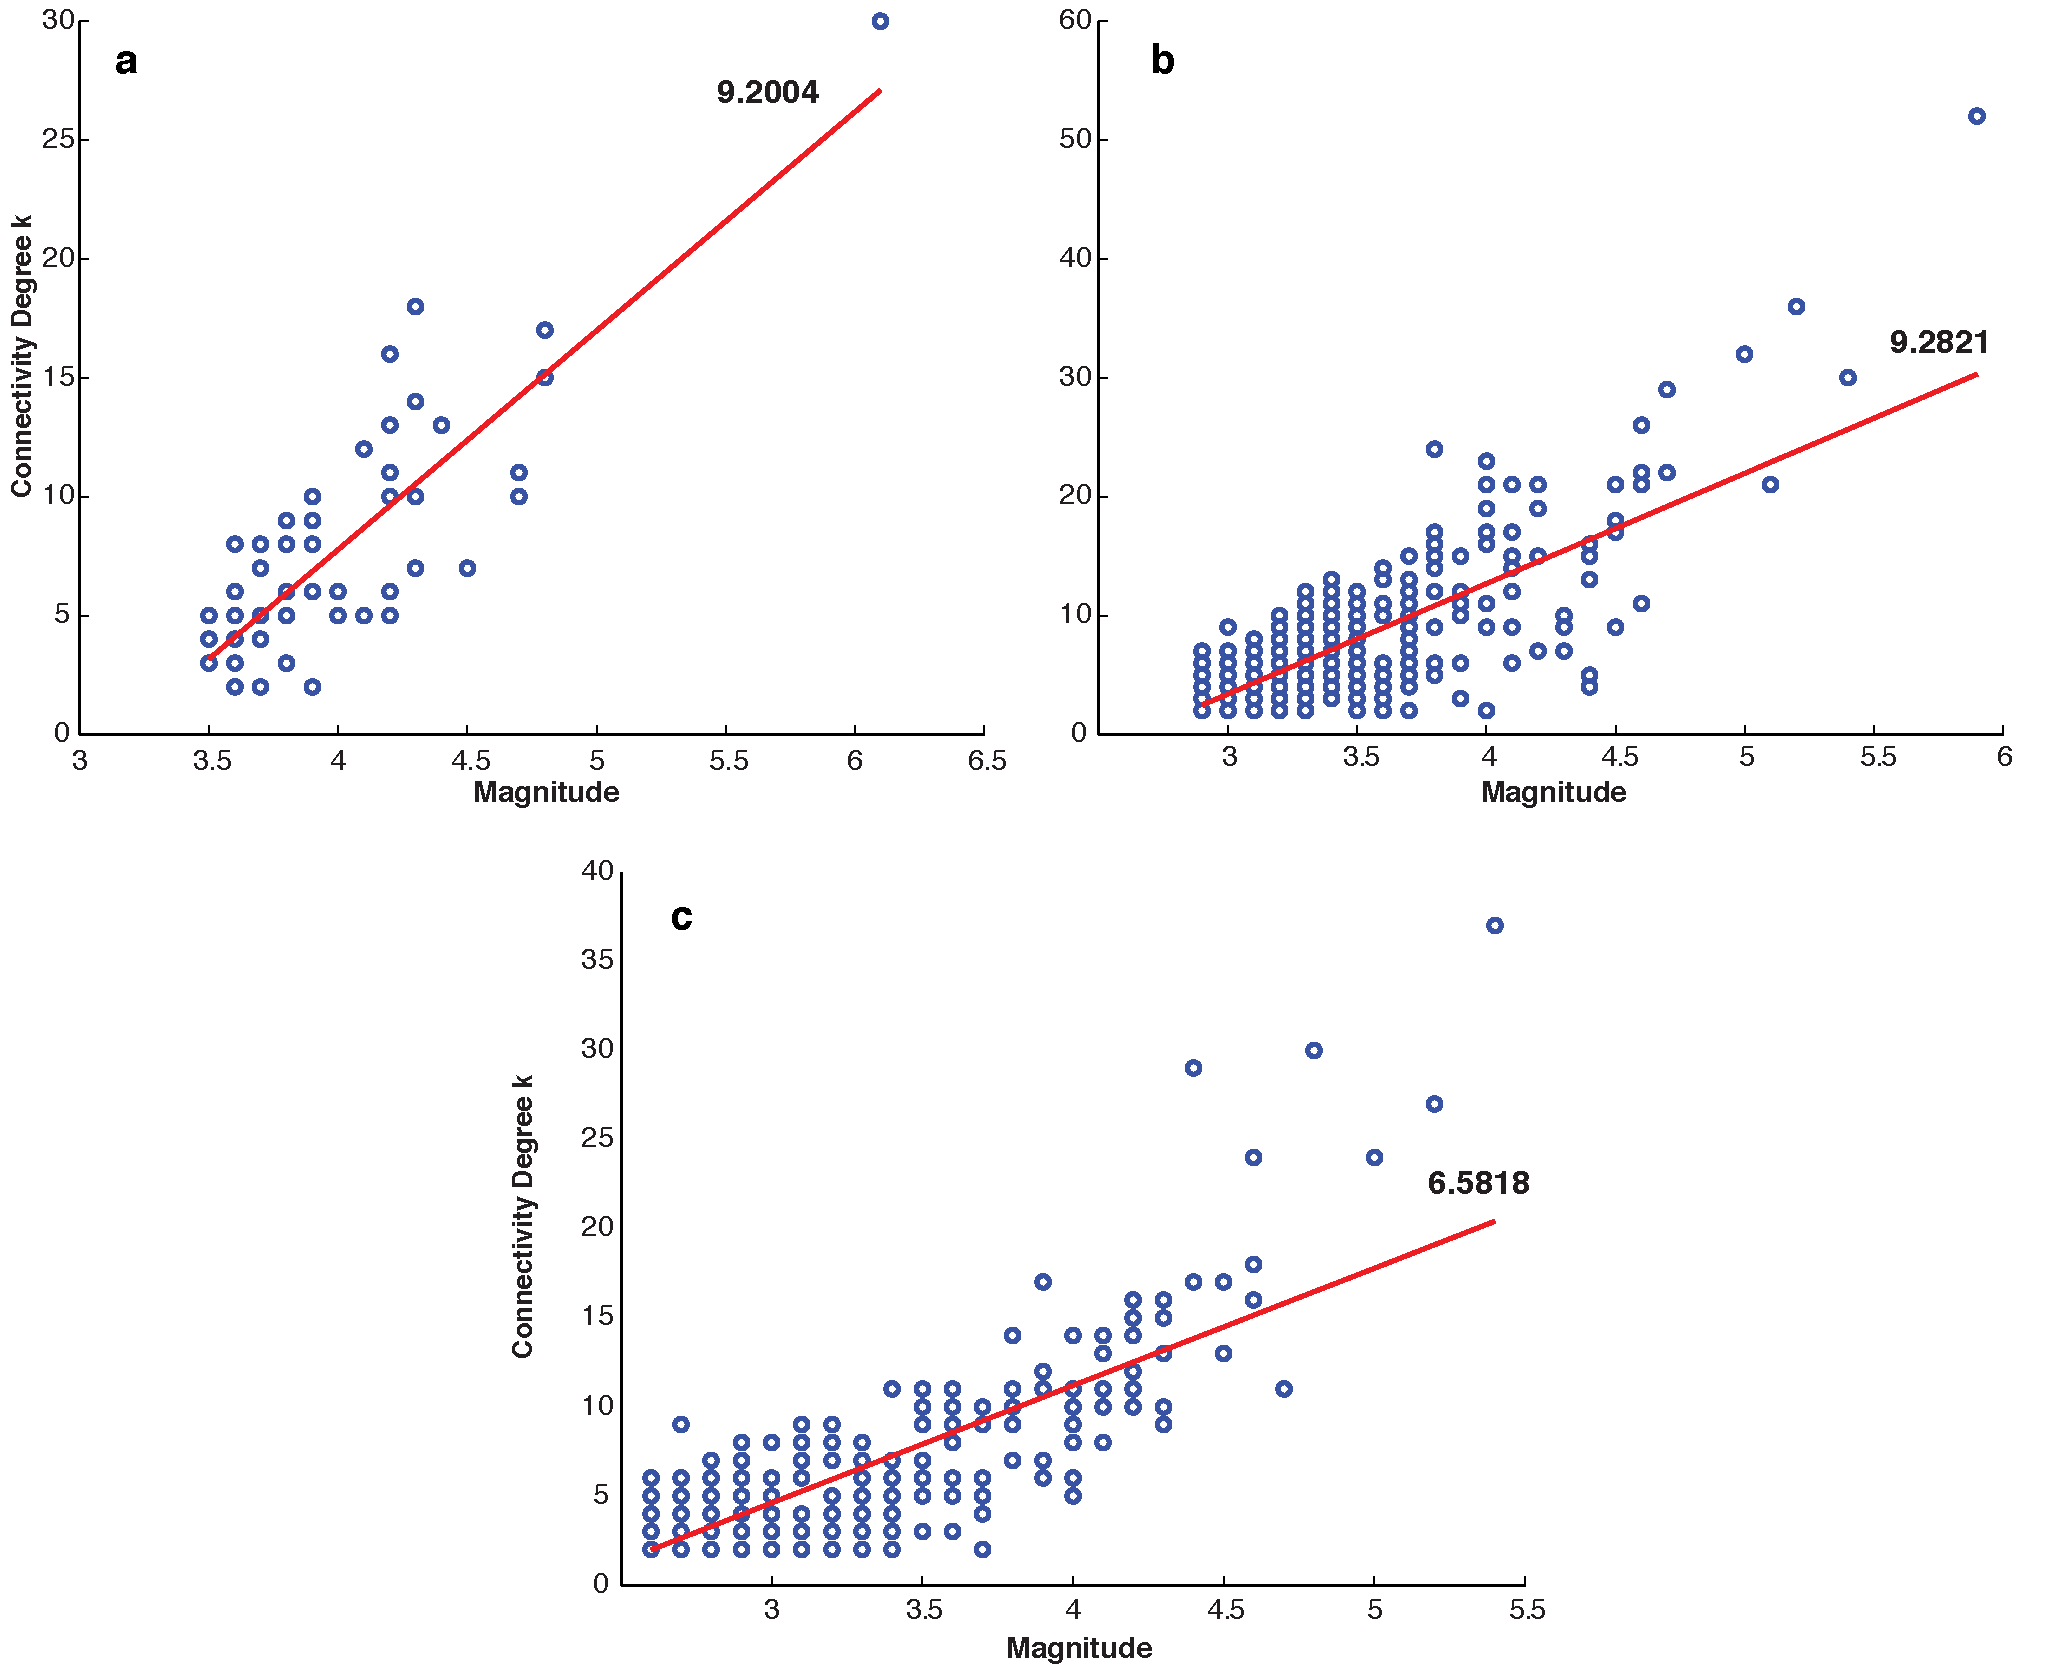
\includegraphics[scale=0.35]{figures/pdf/Figure05.pdf} 
\caption{ K-M relationship for north Iran seismicity. a) Azerbaijan b) Alborz c)Kopeh Dagh}
\label{fig:k_m_plot_m}
\end{figure}

\noindent
We compared the $k-M$ slope with the $b-value$ of the Gutenberg-Richter law in the whole catalog and also in the sliding window in time. The $b-value$ is generated through the maximum likelihood estimation \citep{Aki1965}.

\begin{equation}
b = \frac{log_{10}(e) }{\overline{M} - M_{min}}  
\end{equation}
 
 \noindent
 where $\overline{M}$ is the average magnitude and $M_{min}$ is the minimum magnitude in the sample, which in this case is the completeness magnitude for each tectonic seismic zone. Number of sequences and threshold magnitude are considerably different for all tectonic seismic zones. \citet{Telesca2013} studied the effect of number of earthquake in catalog on the $k-M$ slop. Comparing the result of Guerrero region with reduced random sequence, \citet{Telesca2013} found that the number of sequence doesn't affect the $k-M$ slope.  According to \citet{Telesca2012}, the threshold magnitude has a minor effect in the VG parameters. In order to analyze the sensitivity of the catalogs to the number of events and the threshold magnitude we randomly picked 200 sequence from the catalogs with various sequence size. The minimum size of random windows are 150 events (note that the number of events in each catalog, before removing the events with magnitude less than completeness magnitude, are 271, 1262, and 399 for Azerbaijan, Alborz, and Kopek Dagh regions, respectively) and the maximum size is the whole catalog. For each randomly picked magnitude time series we estimated the $Mc$ and calculated the $k-M$ and $b-value$. Fig.~\ref{fig:random} shows the relationship between $k-M$ slope and $b-value$ of the randomly selected data and statistical parameters for variables. Although changing number of events and the threshold magnitude are slightly change the results, they are fairly well clustered for each tectonic seismic region. 
 
 \begin{figure} [ht]
\centering
\includegraphics[scale=0.3]{figures/pdf/Figure066.pdf} 
\caption{ Relationship between $K-M$ and $b-value$ of three Iranian tectonic seismic zones (this study) and two other studies of Mexican zones \citep{Telesca2013}, and Pannonia zones \citep{Telesca2014}. The dashed red line shows the regression line for data of  Mexican zones and Pannonia zones \citep{Telesca2014}, and the solid blue line shows the regression line for data of all regions (Mexican, Pannonian and North Iran)}
\label{fig:random}
\end{figure}
 
 \noindent
The $k-M$ slope shows the maximum coefficient of variation. We may argue that the $k-M$ slope is much dependent to the window size and threshold magnitude than $a-$ and $b-value$, which suggest the idea that $k-M$ slop can better represent the dynamic characteristics of the magnitude-time series. 
 
 

 
 \noindent
 Fig.~\ref{fig:regression} shows the relationship between the $k-M$ slope for three tectonic seismic zones in Iran and two other studies of Mexican zones \citep{Telesca2013}, and Pannonia zones \citep{Telesca2014}. Adding the results of this study into two previous similar studies' results, improves the regression factor (increase from R=0.95 to R=0.958) and empower the idea of universal character of the relationship between the $b-value$ and the $k-M$ slope as \citet{Telesca2014} concluded. 

\begin{figure} [ht]
\centering
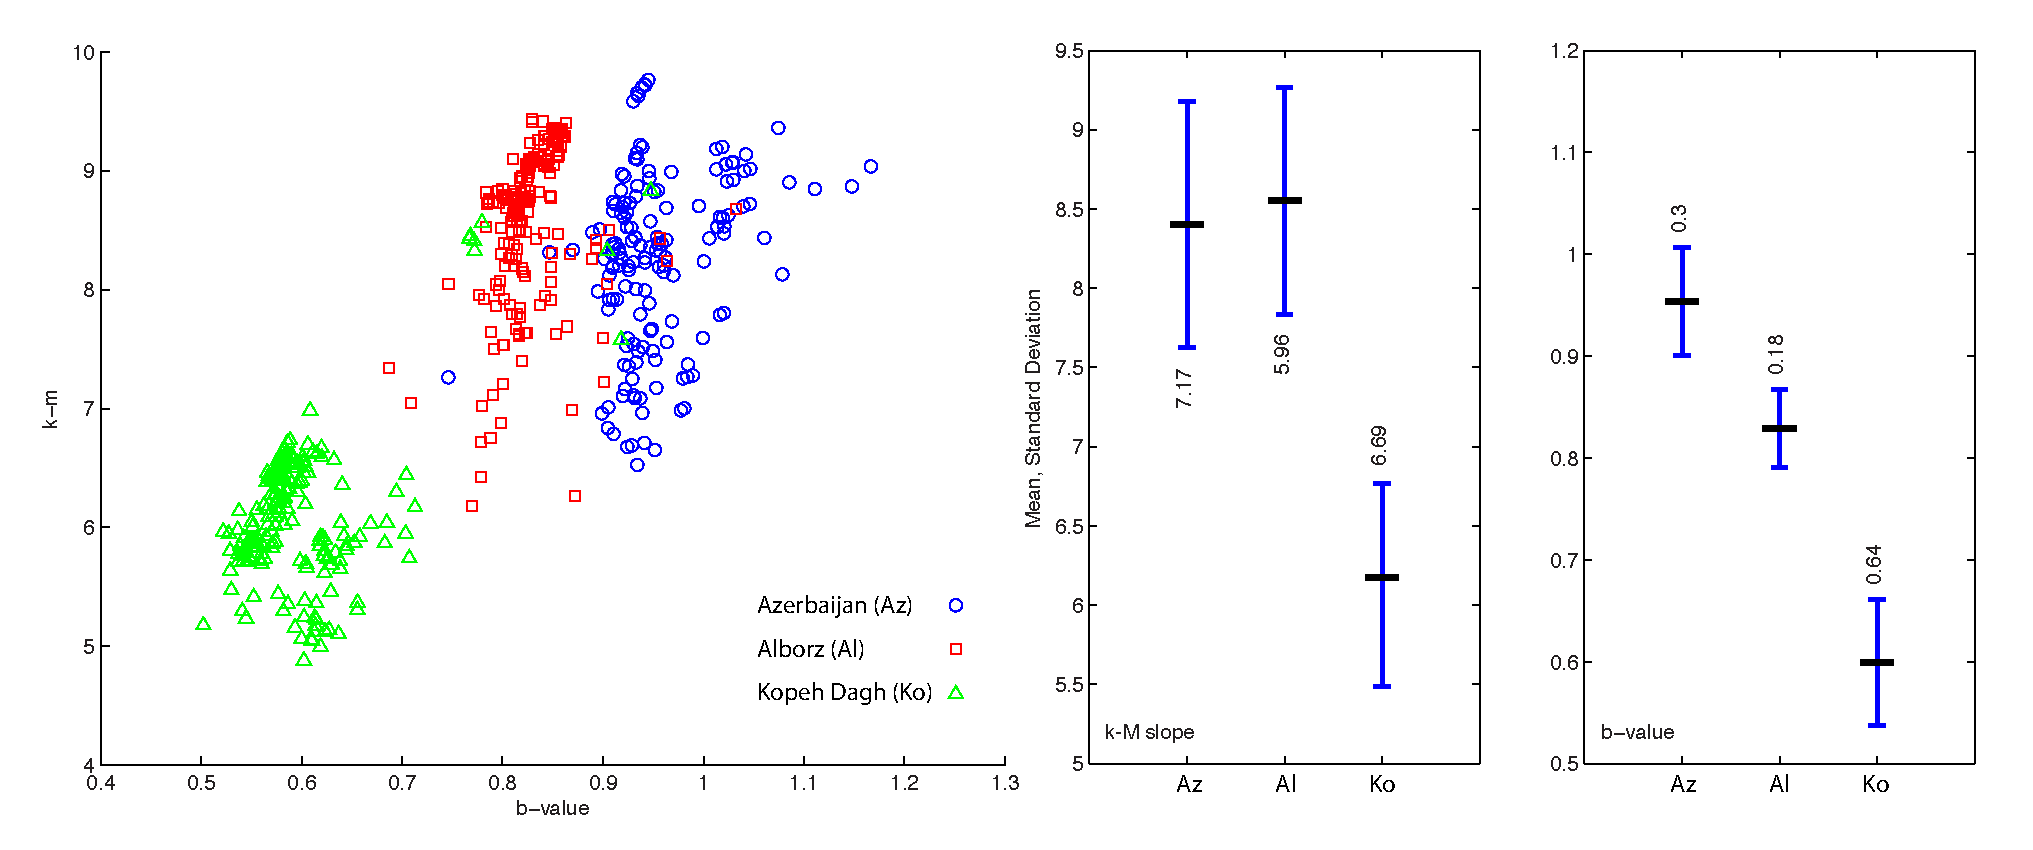
\includegraphics[scale=0.3]{figures/pdf/Figure06.pdf} 
\caption{ Relationship between $K-M$ and $b-value$ of three Iranian tectonic seismic zones (this study) and two other studies of Mexican zones \citep{Telesca2013}, and Pannonia zones \citep{Telesca2014}. The dashed red line shows the regression line for data of  Mexican zones and Pannonia zones \citep{Telesca2014}, and the solid blue line shows the regression line for data of all regions (Mexican, Pannonian and North Iran)}
\label{fig:regression}
\end{figure}

\noindent
The relationship between $b-value$ and $K-M$ slope for Azerbaijan and Alborz region, suggested the idea of similar tectonic activity in these zones, in contrast with the $b-value$. In other words, may $K-M$ slope is more robust and less sensitive than $b-value$. Adding the value of this study into two previous similar studies results improves the regression factor (increase from R=0.95 to R=0.958) and empower the idea of universal character of the relationship between the $b-value$ and the $k-M$ slope as \citet{Telesca2014} pointed out. 





\noindent 
Fig.\ref{fig:tc}  shows the variation of the $k-M$ slope and $b-value$ with time. Having lower number of event, we used 40 events as a window length. We analyzed the sensitivity of the results to the window size. Even though there is a very good similarity between the $K-M$ slope and $b-value$ in Alborz tectonic seismic region, there is no as good as fit for Azerbaijan Tectonic seismic region. The results indicate the fact that, $K-M$ slope may provide extra information about the seismic sequence of the region than the $b-value$. 
 
The value of the K-M is increasing with increasing the magnitude. Fig yy shows the time vacation of the $K-M$ plot and $b-value$ for all tectonic seismic regions. 

In general, In all regions the $b-value$ and $K-M$ slope considerably drops before  big earthquakes. Dropping the $b-value$ before large earthquakes have been studied in many different region \citep[e.g.][]{Wyss2000,Wyss2006,Schorlemmer2005,Chan2012}


Earthquake is a time dependent phenomenon, so studying the dynamic properties of the earthquake sequence is important to get different time dependent parameters. 

 \citet{Telesca2016} observed the decreasing of the $<Tc>$ before large earthquake of Western India earthquake sequence. Fig.~\ref{fig:tc} shows the time variation of $<Tc>$ in the study area. The decreasing of the $<Tc>$ for large earthquakes have been shown in the figure. \citet{Telesca2016} demonstrated that the decrement of $<Tc>$ before large earthquake are independent of window size and the threshold magnitude. 
 
The fluctuation of magnitude time series' topology properties (e.g. the $k-M$ slope and $<Tc>$) could be affected by the window size. Sharp changes in the VG parameters happens through small windows. Using higher number of samples in the window will reduce the temporal effects of small or moderate earthquakes and highlight the effects of big earthquakes, even though the behavior of the parameters in time and also before big earthquake are similar \citep{Telesca2016}. In general, more number of samples in a window smooth the results. 
 
 In this study with increasing window size we can see the same behavior as small window. Undoubtedly, larger window size will reduce the effect of 
 
 
 
 \begin{figure} [ht]
\centering
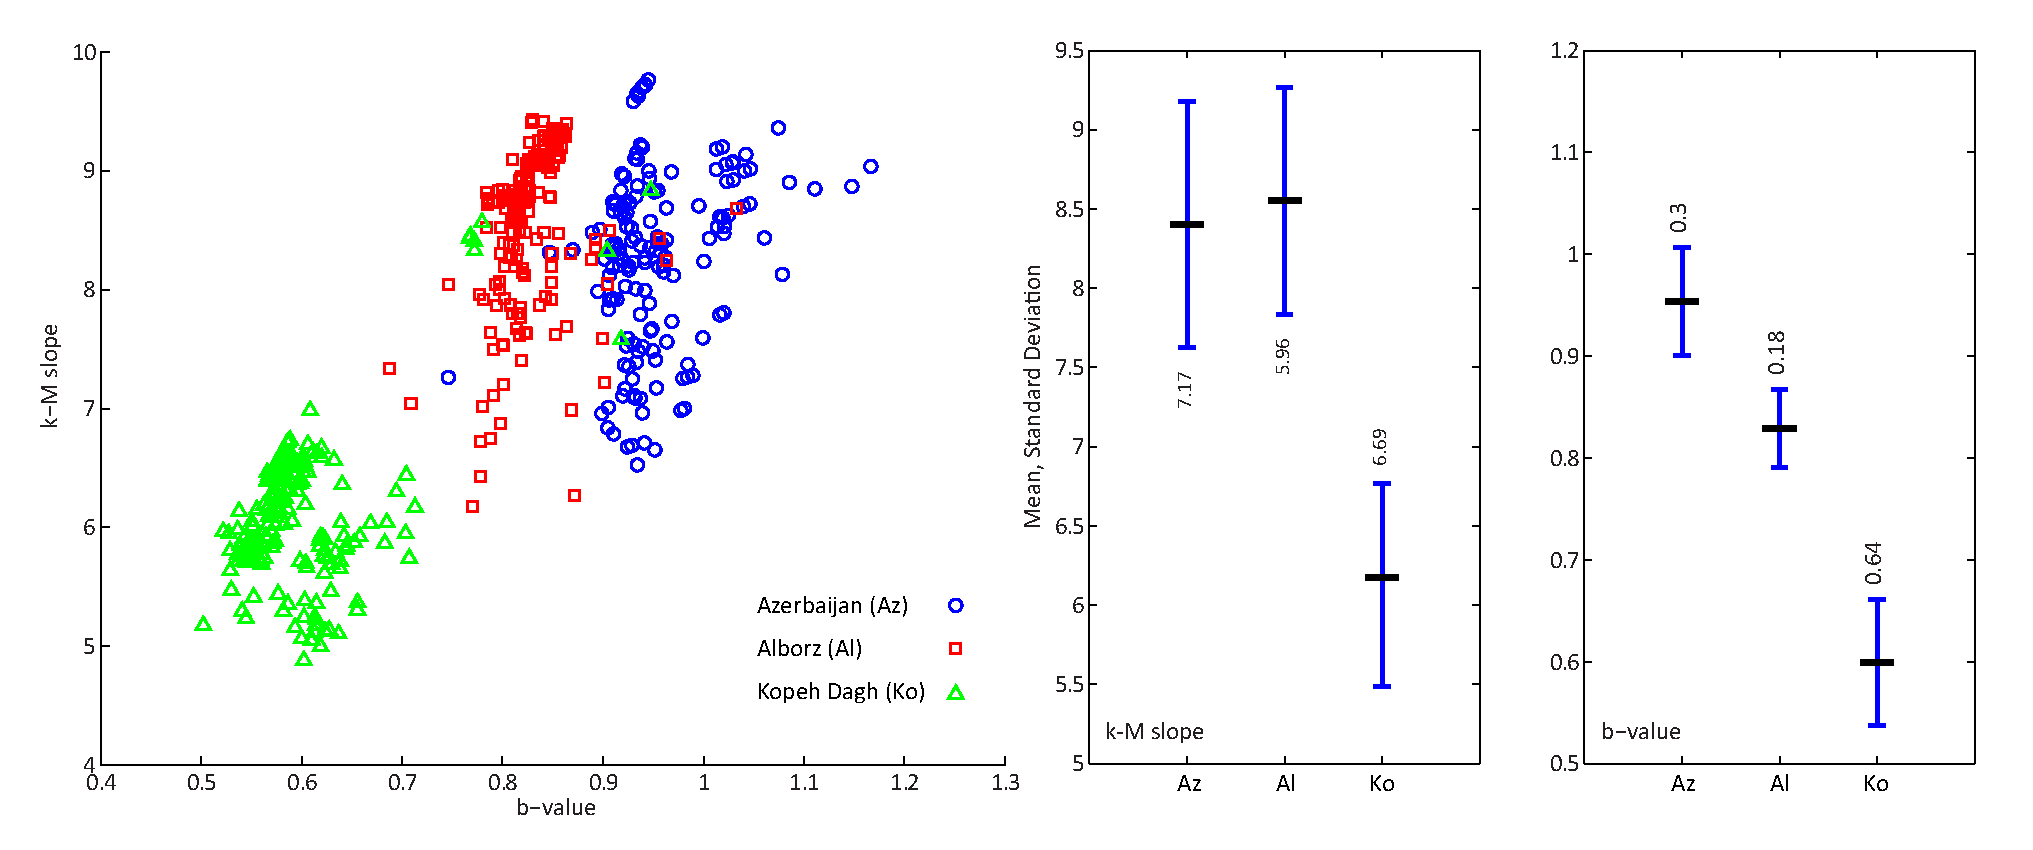
\includegraphics[scale=0.34]{figures/pdf/Figure07.pdf} 
\caption{ Relationship between $K-M$ and $b-value$ of three Iranian tectonic seismic zones (this study) and two other studies of Mexican zones \citep{Telesca2013}, and Pannonia zones \citep{Telesca2014}. The dashed red line shows the regression line for data of  Mexican zones and Pannonia zones \citep{Telesca2014}, and the solid blue line shows the regression line for data of all regions (Mexican, Pannonian and North Iran)}
\label{fig:tc}
\end{figure}
 
 
 
 
 
 
 